\documentclass[11pt,a4paper]{article}

\usepackage[utf8]{inputenc}
\usepackage[spanish,es-nodecimaldot]{babel}
\usepackage[T1]{fontenc}
\usepackage{lmodern}
\usepackage{geometry}
\geometry{top=2.5cm, bottom=2.5cm, left=2.5cm, right=2.5cm}

\usepackage{amsmath,amssymb}
\usepackage{graphicx}
\usepackage{booktabs}
\usepackage{float}
\usepackage{hyperref}
\hypersetup{colorlinks=true, linkcolor=black, urlcolor=blue}

\setlength{\parindent}{0pt}
\setlength{\parskip}{6pt}

\title{
    \vspace{-1.2cm}
    \textbf{Sistemas de Control}\\
    \large Trabajo de Laboratorio Integrador: Desarrollo de Controladores\\
    \normalsize Segunda Parte: Control Proporcional-Integral (PI)
}
\author{Tomás Gómez Pizarro \quad\and\quad Mikael Rodríguez}
\date{Noviembre 2026}

\begin{document}

\maketitle

\section*{Segunda parte: Control proporcional-integral}

Se implementa un controlador proporcional-integral (PI) para intentar satisfacer simultáneamente las tres especificaciones de diseño en lazo cerrado:
\begin{itemize}
    \item $PO \le 5\%$
    \item $T_s \le 0{,}10\text{ s}$ (criterio del $2\%$)
    \item $e_{ss} = 0$ ante escalón unitario
\end{itemize}

La función de transferencia del controlador es:
\begin{equation}
    G_c(s) = \frac{k_p s + k_i}{s} = k_p \frac{s + z}{s}, \quad \text{con } z = \frac{k_i}{k_p}
\end{equation}

\subsection*{Punto 1. Condiciones de estabilidad mediante el criterio de Routh}

La función de transferencia de lazo abierto con el controlador PI resulta:
\begin{equation}
    L(s) = G_c(s) G(s) = \frac{k_p s + k_i}{s (\tau_1 s + 1)(\tau_2 s + 1)}
\end{equation}
donde $\tau_1 = R_1 C_1 = 0{,}01\text{ s}$ y $\tau_2 = R_2 C_2 = 0{,}0047\text{ s}$. La ecuación característica de lazo cerrado es:
\begin{equation}
    1 + L(s) = 0 \implies s (\tau_1 s + 1)(\tau_2 s + 1) + (k_p s + k_i) = 0
\end{equation}
Desarrollando los productos:
\begin{equation}
    \tau_1 \tau_2 s^3 + (\tau_1 + \tau_2) s^2 + (1 + k_p) s + k_i = 0
\end{equation}
Reemplazando los valores numéricos ($\tau_1 \tau_2 = 4{,}7\times 10^{-5}\text{ s}^2$ y $\tau_1 + \tau_2 = 0{,}0147\text{ s}$):
\begin{equation}
    4{,}7\times 10^{-5} s^3 + 0{,}0147 s^2 + (1 + k_p) s + k_i = 0
\end{equation}

Construyendo la tabla de Routh-Hurwitz para este polinomio de tercer orden:
\begin{table}[H]
\centering
\begin{tabular}{c | c c}
$s^3$ & $\tau_1 \tau_2$ & $1 + k_p$ \\
$s^2$ & $\tau_1 + \tau_2$ & $k_i$ \\
$s^1$ & $b_1$ & $0$ \\
$s^0$ & $k_i$ & 
\end{tabular}
\end{table}

donde el coeficiente de la fila $s^1$ es:
\begin{equation}
    b_1 = \frac{(\tau_1 + \tau_2)(1 + k_p) - \tau_1 \tau_2 k_i}{\tau_1 + \tau_2}
\end{equation}

Para que todos los polos se ubiquen en el semiplano izquierdo, no debe haber cambios de signo en la primera columna, lo que exige:
\begin{enumerate}
    \item De la fila $s^0$:
    \begin{equation}
        k_i > 0
    \end{equation}
    \item De la fila $s^1$:
    \begin{equation}
        b_1 > 0 \implies k_i < \frac{\tau_1 + \tau_2}{\tau_1 \tau_2} (1 + k_p)
    \end{equation}
\end{enumerate}

Evaluando el factor numérico:
\begin{equation}
    \frac{\tau_1 + \tau_2}{\tau_1 \tau_2} = \frac{0{,}0147}{4{,}7\times 10^{-5}} \approx 312{,}77\text{ rad/s}
\end{equation}
Por ende, las condiciones necesarias y suficientes para la estabilidad en lazo cerrado son:
\begin{equation}
    k_i > 0 \quad \text{y} \quad k_i < 312{,}77 \cdot (1 + k_p)
\end{equation}
Físicamente, esto indica que existe un límite superior para la ganancia integral $k_i$; si se supera esta cota, la acción integral introduce un retardo de fase excesivo que desestabiliza el sistema.

\subsection*{Punto 2. Diseño del PI mediante el Lugar de las Raíces}

\subsubsection*{2.a. Requisitos en el plano $s$}
\begin{itemize}
    \item \textbf{Sobrepaso ($PO \le 5\%$):} Para un sistema canónico de segundo orden, el amortiguamiento mínimo requerido es:
    \begin{equation}
        \xi \ge \frac{-\ln(0{,}05)}{\sqrt{\pi^2 + \ln^2(0{,}05)}} \approx 0{,}69
    \end{equation}
    Esto delimita en el plano complejo un cono admisible con semiángulo respecto al eje real negativo de:
    \begin{equation}
        \theta = \arccos(0{,}69) \approx 46{,}4^\circ
    \end{equation}
    \item \textbf{Tiempo de establecimiento ($T_s \le 0{,}10\text{ s}$ al $2\%$):} La cota impone:
    \begin{equation}
        T_s \approx \frac{4}{\xi\omega_n} \le 0{,}10\text{ s} \implies \xi\omega_n \ge 40\text{ rad/s}
    \end{equation}
    Los polos dominantes deben quedar a la izquierda de la recta vertical $\text{Re}(s) = -40\text{ rad/s}$.
\end{itemize}

\begin{figure}[H]
    \centering
    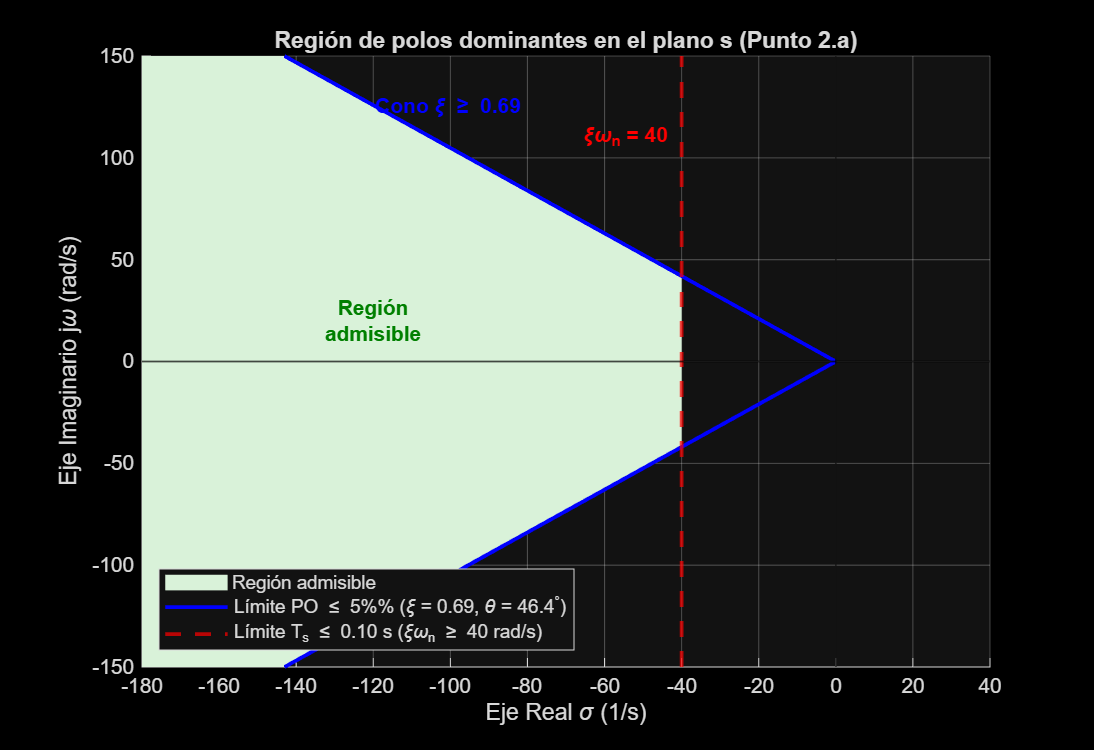
\includegraphics[width=0.65\textwidth]{figuras/pi_punto2a_region_s.png}
    \caption{Región admisible para los polos dominantes en el plano $s$ delimitada por $PO \le 5\%$ (cono $\xi \ge 0{,}69$) y $T_s \le 0{,}10\text{ s}$ (semiplano $\xi\omega_n \ge 40\text{ rad/s}$).}
    \label{fig:pi_region_s}
\end{figure}

\subsubsection*{2.b. Centro de las asíntotas $\sigma_a$ en función de $z$}
La función de lazo abierto $L(s) = k_p \frac{s + z}{s(\tau_1 s + 1)(\tau_2 s + 1)}$ posee $n = 3$ polos ($0, -100, -212{,}77\text{ rad/s}$) y $m = 1$ cero en $-z$. Al haber un exceso de dos polos sobre ceros ($n - m = 2$), existen dos ramas que tienden al infinito a lo largo de asíntotas cuyos ángulos están dados por:
\begin{equation}
    \phi_k = \frac{(2k + 1) \cdot 180^\circ}{n - m} = \frac{(2k + 1) \cdot 180^\circ}{2} \implies \phi_0 = 90^\circ, \quad \phi_1 = 270^\circ \equiv -90^\circ
\end{equation}
Dado que los ángulos son exactamente $\pm 90^\circ$, las asíntotas son \textbf{estrictamente verticales} (perpendiculares al eje real). Su punto de partida sobre el eje real es el centro de asíntotas:
\begin{equation}
    \sigma_a = \frac{\sum \text{polos} - \sum \text{ceros}}{n - m} = \frac{(0 - 100 - 212{,}77) - (-z)}{2} = \frac{z - 312{,}77}{2}
\end{equation}

Para que las asíntotas queden a la izquierda de la cota $\text{Re}(s) = -40\text{ rad/s}$:
\begin{equation}
    \sigma_a < -40 \implies \frac{z - 312{,}77}{2} < -40 \implies z < 312{,}77 - 80 \implies z < 232{,}77\text{ rad/s}
\end{equation}

\subsubsection*{2.c. Elección de la posición del cero $z$ y diseño preliminar}
Para la elección del cero $z$, si bien cualquier valor en el intervalo $0 < z < 232{,}77\text{ rad/s}$ cumple formalmente la condición del centroide de asíntotas ($\sigma_a < -40\text{ rad/s}$), la distribución de las ramas del Lugar de las Raíces sobre el eje real impone una restricción de diseño fundamental:
\begin{itemize}
    \item \textbf{Descarte de $z < 100\text{ rad/s}$:} En esta región, el segmento $[-z,\, 0]$ pertenece al Lugar de las Raíces. La rama que parte del polo en el origen ($s = 0$) termina en el cero en $s = -z$ sobre el eje real, dejando un polo real de lazo cerrado atrapado entre $0$ y $-z$. Al quedar este polo real más próximo al eje imaginario que las ramas complejas, pasa a ser el polo dominante del sistema. Esto invalida la aproximación de segundo orden y anula la posibilidad de lograr el factor de amortiguamiento deseado ($\xi = 0{,}69$) a través del par complejo.
    \item \textbf{Elección con $z \ge 100\text{ rad/s}$:} En este caso, el segmento del eje real que pertenece al Lugar de las Raíces es $[-100,\, 0]$. Las dos ramas que parten de $0$ y $-100\text{ rad/s}$ colisionan en un punto de ruptura y emergen al plano complejo, constituyendo el par complejo dominante con el amortiguamiento deseado. A su vez, la rama que parte del polo en $-212{,}77\text{ rad/s}$ termina en el cero en $-z$, confinando el polo real a la izquierda de $-z$, donde decae rápidamente sin distorsionar la dinámica del par complejo.
\end{itemize}

\textbf{Evaluación de la alternativa de cancelación polo-cero ($z = 100\text{ rad/s}$):}
Se analizó la posibilidad de adoptar $z = 100\text{ rad/s}$ para cancelar el polo de la planta en $s = -100\text{ rad/s}$, reduciendo el sistema a segundo orden con polos en $0$ y $-212{,}77\text{ rad/s}$ y punto de ruptura en $\sigma = -106{,}38\text{ rad/s}$ ($T_s \approx 38\text{ ms}$). Incluso ante tolerancias reales de componentes ($z \approx 100$), el residuo de la fracción simple del polo imperfectamente cancelado es proporcional a $(z - 100)$, resultando en una amplitud transitoria casi nula. Sin embargo, se descartó este camino porque al eliminar algebraicamente el cero se suprime la dependencia paramétrica de $\sigma_a(z)$ deducida en el Punto 2.b y se pierde la presencia del cero en lazo cerrado cuyo efecto sobre el sobrepaso se solicita evaluar en el Punto 2.d.

Por ello, para satisfacer simultáneamente la cota de las asíntotas ($\sigma_a < -40\text{ rad/s} \implies z < 232{,}77\text{ rad/s}$) y asegurar que el par complejo domine la dinámica sin depender de cancelaciones algebraicas, se adopta:
\begin{equation}
    z = 120\text{ rad/s}
\end{equation}
Con este valor, el centro de las asíntotas se sitúa en $\sigma_a = (120 - 312{,}77)/2 = -96{,}38\text{ rad/s} \ll -40\text{ rad/s}$.

Trazando el Lugar de las Raíces con $z = 120\text{ rad/s}$ en MATLAB (Figura \ref{fig:pi_lgr}) y mediante la selección interactiva sobre la cota de amortiguamiento $\xi = 0{,}69$, se obtiene la ganancia inicial:
\begin{equation}
    k_p \approx 0{,}84 \implies k_i = k_p \cdot z = 0{,}84 \times 120 \approx 100{,}8\text{ rad/s}
\end{equation}
con polos en lazo cerrado en:
\begin{equation}
    s_{1,2} \approx -83{,}9 \pm j 88{,}2\text{ rad/s} \quad (\xi = 0{,}690), \qquad s_3 \approx -144{,}6\text{ rad/s}
\end{equation}

\begin{figure}[H]
    \centering
    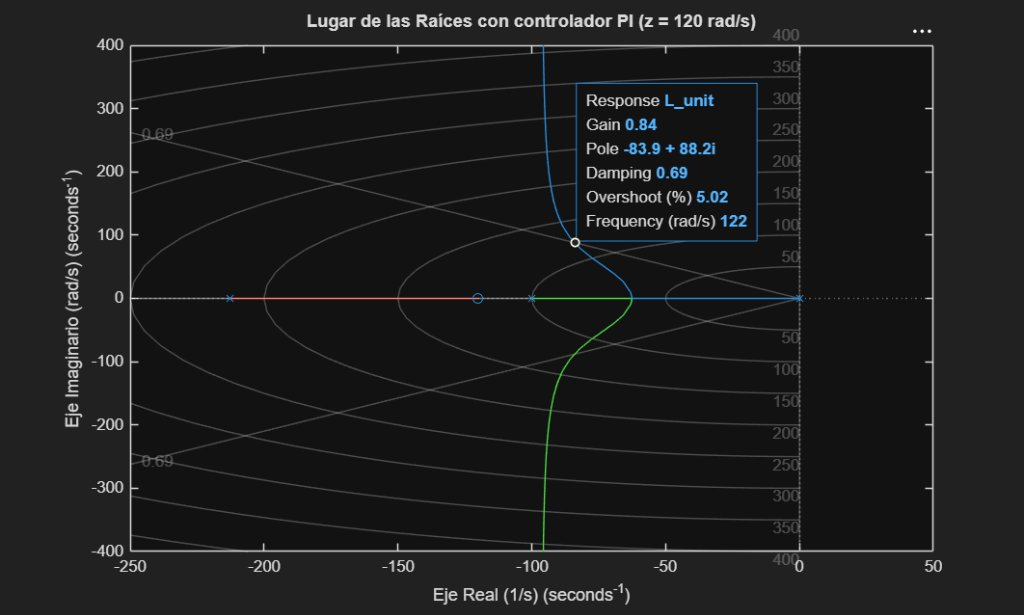
\includegraphics[width=0.75\textwidth]{figuras/pi_punto2_lgr.png}
    \caption{Lugar de las Raíces con controlador PI ($z = 120\text{ rad/s}$) en MATLAB y selección interactiva de $k_p = 0{,}84$ sobre la cota $\xi = 0{,}69$.}
    \label{fig:pi_lgr}
\end{figure}

\subsubsection*{2.d. Efecto del cero en lazo cerrado y ajuste de $k_p$}
La evaluación de la respuesta al escalón con $k_p = 0{,}84$ arroja:
\begin{itemize}
    \item $PO = 6{,}79\% > 5\%$ \quad $\rightarrow$ \textbf{No cumple}.
    \item $T_s = 48{,}9\text{ ms} \le 100\text{ ms}$ \quad $\rightarrow$ \textbf{Cumple}.
    \item $e_{ss} = 0$ \quad $\rightarrow$ \textbf{Cumple}.
\end{itemize}

\textbf{Causa del sobrepaso adicional:} La función de transferencia de lazo cerrado es:
\begin{equation}
    T(s) = \frac{k_p(s + z)}{\tau_1\tau_2 s^3 + (\tau_1+\tau_2)s^2 + (1+k_p)s + k_i}
\end{equation}
El cero del controlador en $s = -z = -120\text{ rad/s}$ se conserva en el numerador. En el dominio temporal, un término de la forma $(1 + s/z)$ equivale a sumar a la respuesta un término proporcional a su derivada temporal:
\begin{equation}
    y(t) = y_{\text{proto}}(t) + \frac{1}{z} \frac{d y_{\text{proto}}(t)}{dt}
\end{equation}
Durante la etapa de subida, la derivada es estrictamente positiva, lo que anticipa la llegada al valor final y eleva el pico máximo respecto al modelo canónico de segundo orden sin ceros (donde $\xi = 0{,}69$ produce teóricamente un $PO \approx 4{,}99\%$). La Figura \ref{fig:pi_efecto_cero} muestra la comparación temporal entre el prototipo puro de segundo orden y el sistema real.

\begin{figure}[H]
    \centering
    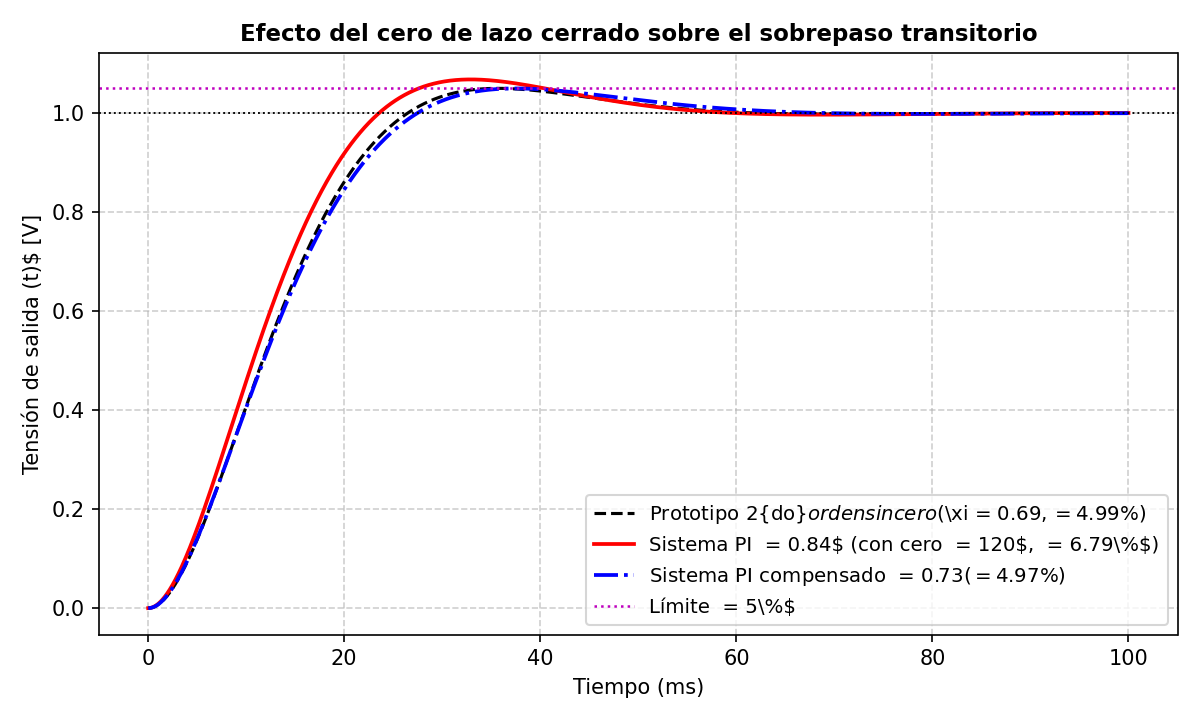
\includegraphics[width=0.75\textwidth]{figuras/pi_punto2_efecto_cero.png}
    \caption{Efecto del cero de lazo cerrado en $s = -120\text{ rad/s}$ sobre la respuesta al escalón y compensación mediante el ajuste fino de ganancia a $k_p = 0{,}73$.}
    \label{fig:pi_efecto_cero}
\end{figure}

\textbf{Compensación de la ganancia:} Para reducir el sobrepaso por debajo del $5\%$, se realiza un ajuste fino iterativo disminuyendo progresivamente la ganancia sobre el Lugar de las Raíces. Se comprueba empíricamente que con:
\begin{equation}
    k_p = 0{,}73 \implies k_i = 0{,}73 \times 120 = 87{,}6\text{ rad/s}
\end{equation}
el sistema calza justo en el límite de la especificación dinámica requerida maximizando el ancho de banda, con polos en $s_{1,2} \approx -81{,}2 \pm j 76{,}2\text{ rad/s}$ ($\xi \approx 0{,}729$) y $s_3 \approx -150{,}5\text{ rad/s}$. Las métricas temporales resultan:
\begin{itemize}
    \item $PO = 4{,}97\% \le 5\%$ \quad $\rightarrow$ \textbf{Cumple} (calza en la cota admisible).
    \item $T_s = 52{,}8\text{ ms} \le 100\text{ ms}$ \quad $\rightarrow$ \textbf{Cumple}.
    \item $e_{ss} = 0$ \quad $\rightarrow$ \textbf{Cumple}.
\end{itemize}

\subsection*{Punto 3. Implementación del controlador con amplificadores operacionales}

\subsubsection*{3.a. Deducción de la función de transferencia del circuito PI (Figura 3)}
El circuito de la Figura 3 corresponde a un amplificador inversor con una impedancia de entrada puramente resistiva $Z_{\text{in}}(s) = R_{PI1}$ y una impedancia de realimentación serie formada por $R_{PI2}$ y $C_{PI}$:
\begin{equation}
    Z_f(s) = R_{PI2} + \frac{1}{C_{PI} s} = \frac{R_{PI2} C_{PI} s + 1}{C_{PI} s}
\end{equation}
Bajo las hipótesis de operacional ideal ($i_+ = i_- = 0$, $v_+ = v_- = 0\text{ V}$), planteando la ley de corrientes en el nodo inversor:
\begin{equation}
    \frac{V_i(s)}{R_{PI1}} + \frac{V_{o1}(s)}{Z_f(s)} = 0 \implies \frac{V_{o1}(s)}{V_i(s)} = -\frac{Z_f(s)}{R_{PI1}} = -\left( \frac{R_{PI2}}{R_{PI1}} + \frac{1}{R_{PI1} C_{PI} s} \right)
\end{equation}
Factorizando:
\begin{equation}
    \frac{V_{o1}(s)}{V_i(s)} = -\frac{\frac{R_{PI2}}{R_{PI1}} s + \frac{1}{R_{PI1} C_{PI}}}{s}
\end{equation}
Queda demostrado que la etapa implementa un controlador PI inversor, con parámetros:
\begin{equation}
    k_p = \frac{R_{PI2}}{R_{PI1}}, \qquad k_i = \frac{1}{R_{PI1} C_{PI}}, \qquad z = \frac{k_i}{k_p} = \frac{1}{R_{PI2} C_{PI}}
\end{equation}

\subsubsection*{3.b. Dimensionamiento con valores comerciales (serie E24)}
Para cancelar la inversión de signo se coloca a continuación la etapa inversora unitaria de la Figura 4:
\begin{equation}
    \frac{V_{PI}(s)}{V_{o1}(s)} = -\frac{R_{INV2}}{R_{INV1}} = -1 \implies R_{INV1} = R_{INV2} = 10\text{ k}\Omega \quad (\text{E24})
\end{equation}
Fijando el capacitor en $C_{PI} = 0{,}1\,\mu\text{F}$ según la consigna, se dimensionan los resistores de la etapa PI:
\begin{itemize}
    \item Para ubicar el cero en $z \approx 120\text{ rad/s}$:
    \begin{equation}
        R_{PI2} = \frac{1}{z \cdot C_{PI}} = \frac{1}{120 \times 0{,}1\times 10^{-6}} = 83{,}33\text{ k}\Omega \implies \mathbf{R_{PI2} = 82\text{ k}\Omega \quad (\text{E24})}
    \end{equation}
    \item Para aproximar la ganancia de diseño $k_p \approx 0{,}73$ con componentes comerciales:
    \begin{equation}
        R_{PI1} = \frac{R_{PI2}}{k_p} = \frac{82\text{ k}\Omega}{0{,}73} \approx 112{,}33\text{ k}\Omega
    \end{equation}
    En la serie E24, el valor inferior inmediato $110\text{ k}\Omega$ daría $k_p = 82/110 \approx 0{,}7455$, elevando el sobrepaso a $PO = 5{,}70\% > 5\%$. Por lo tanto, con un criterio conservador frente a tolerancias (análogo al adoptado en la Primera Parte), se elige el valor comercial superior:
    \begin{equation}
        \mathbf{R_{PI1} = 120\text{ k}\Omega \quad (\text{E24})}
    \end{equation}
\end{itemize}

Los valores efectivos del controlador con los componentes comerciales adoptados resultan:
\begin{equation}
    k_p = \frac{82\text{ k}\Omega}{120\text{ k}\Omega} = 0{,}6833, \quad k_i = \frac{1}{120\text{ k}\Omega \times 0{,}1\,\mu\text{F}} = 83{,}33\text{ rad/s}, \quad z = \frac{83{,}33}{0{,}6833} = 121{,}95\text{ rad/s}
\end{equation}


Todos los cálculos y figuras de esta sección se generan ejecutando el script \texttt{TP\_Lab2.m}.

\end{document}
